\documentclass[a4paper,12pt]{article} 
% 使用ctex包支持中文
\usepackage[UTF8,heading = true]{ctex}
\usepackage[utf8]{inputenc}
\usepackage[T1]{fontenc}
\usepackage{graphicx}
\usepackage{float}
\usepackage{amsmath}
\usepackage{amsfonts}
\usepackage{amssymb}
\usepackage{booktabs}
\usepackage{multirow}
\usepackage{subcaption}
\usepackage{indentfirst}
\usepackage{geometry}
\usepackage{fancyhdr}
\usepackage{ctex}
\usepackage[labelfont=bf]{caption}
\usepackage{listings}
\usepackage{xcolor} % 用于定义自定义颜色和高亮
\usepackage{ragged2e} % 导入ragged2e宏包,用于支持段落两端对齐
\usepackage{cite}

\lstset{
  language=Matlab,              % 设置语言为 MATLAB
  basicstyle=\ttfamily\small,   % 设置基本样式
  keywordstyle=\color{blue},    % 设置关键字样式
  stringstyle=\color{red},      % 设置字符串样式
  commentstyle=\color{green},   % 设置注释样式
  morecomment=[l][\color{magenta}]{\%},   % 对行内注释进行高亮
  morecomment=[s][\color{magenta}]{\%\{}{\%\}},   % 对多行注释进行高亮
  frame=single,                 % 给代码添加框
  rulecolor=\color{black},      % 框的颜色
  numbers=left,                 % 在左侧添加行号
  numberstyle=\tiny\color{gray},% 行号样式
  breaklines=true,              % 自动换行
  postbreak=\mbox{\textcolor{red}{$\hookrightarrow$}\space},
  showstringspaces=false,       % 不特别显示字符串中的空格
  tabsize=2                     % 设置tab为2个空格宽度
}



\geometry{left=3cm,right=3cm,top=3cm,bottom=3cm}


\fancyhead{}


\begin{document}

%制作封面
\begin{titlepage}
    \begin{center}
        \par
            \centerline{
\includegraphics[scale=1.5]{data/media/image1.jpeg} 
\includegraphics[scale=3]{data/media/image2.jpeg}} %插入图片
        \par
		\vskip 5cm
		\lishu \fontsize{50}{20} 实\quad 验\quad 报\quad 告
  
		\vskip 2cm
        \lishu \fontsize{35}{20} 实\quad 验\quad 三
        \vskip 5cm

	\begin{tabular}{l}
		\songti \zihao{-2} \bfseries 课程名称:《数字信号处理实验》
		\quad \\
	    	\songti \zihao{-2} \bfseries 学生姓名:邹易航
	    	\quad \\
		\songti \zihao{-2} \bfseries 学生学号:202264691103
		\quad \\
	    	\songti \zihao{-2} \bfseries 学生专业:人工智能
	    	\quad \\
	     \songti \zihao{-2} \bfseries 开课学期:2023-2024年第二学期
	     \quad \\
           \songti \zihao{-2} \bfseries  提交日期:2024年5月25日
    \end{tabular}
    \end{center}
\end{titlepage}


% 生成目录
\newpage
\pagestyle{empty}
\begin{center}
\tableofcontents
\end{center}

\newpage

\setcounter{page}{1}

\section{验证性实验}
\subsection{实验目的}
\begin{itemize}
    \item 求系统的零、极点和幅度频率响应和相位响应。
    \item 求直接型系统函数的零、极点,并转换成二阶节形式
    \item 求差分方程所对应的系统的频率响应。
    \item 设计全通系统,分析系数、零极点、幅频、相频等特性
    \item 分别设计四类线性相位FIR系统,分析系数、零点、幅频、相频等特性
    \cite{ning2012}

\end{itemize}

\subsection{实验原理}
\subsubsection{零点与极点}
零点和极点是描述系统传递函数特性的重要概念。它们直接影响系统的稳定性、频率响应以及时域特性。
\begin{itemize}
    \item \textbf{零点(Zeros)}

    零点是使得系统传递函数为零的值,也就是在零点处系统的输出为零。在复平面上,零点表示为 \( z = z_0 \)。如果一个系统有 \( n \) 个零点,那么传递函数的分子可以写为:
\begin{equation}
    B(z) = (z - z_1)(z - z_2) \cdots (z - z_n)
\end{equation}

其中,\( z_1, z_2, \ldots, z_n \) 是系统的零点。

    \item \textbf{极点(Poles)}

    极点是使得系统传递函数为无穷大的值,也就是在极点处系统的输出趋向于无穷大。在复平面上,极点表示为 \( z = p_0 \)。如果一个系统有 \( m \) 个极点,那么传递函数的分母可以写为:

\begin{equation}
    A(z) = (z - p_1)(z - p_2) \cdots (z - p_m)
\end{equation}

其中,\( p_1, p_2, \ldots, p_m \) 是系统的极点。

    
\end{itemize}

零点与极点具有以下特点:

\begin{itemize}
    \item \textbf{零点和极点的数量相等性:}在线性时不变系统中,系统的零点和极点的数量通常是相等的。这是因为系统的稳定性和因果性要求传递函数的分子和分母次数相等。
    
    \item \textbf{影响频率响应:}零点和极点的位置直接影响系统的频率响应。零点通常表示系统的增益或增益峰值,而极点则表示系统的衰减或衰减谷值。
    
    \item \textbf{系统稳定性:}系统的稳定性与极点的位置有关。如果系统的所有极点都位于单位圆内(在离散时间系统中),系统是稳定的。如果有任何一个极点位于单位圆外,系统就是不稳定的。
\end{itemize}

通过计算传递函数的分子和分母多项式的根,我们可以确定系统的零点和极点的位置。在 Matlab 中,可以使用 \texttt{roots} 函数来找到多项式的根。

\subsubsection{频率幅度响应}
幅度频率响应描述了系统对不同频率输入信号的幅度变化情况。在离散时间系统中,可以通过频率响应函数的幅度来描述系统对不同频率的衰减或增益情况。

通常情况下,系统的传递函数 \( H(z) \) 可以表示为分子 \( B(z) \) 与分母 \( A(z) \) 的比值:
\begin{equation}
    H(z) = \frac{B(z)}{A(z)}
\end{equation}

系统的频率响应可以通过传递函数的频率响应来计算。在离散时间系统中,频率响应可以通过将 \( z \) 替换为单位圆上的点 \( e^{j\omega} \) 来得到:

\begin{equation}
    H(e^{j\omega}) = \frac{B(e^{j\omega})}{A(e^{j\omega})}
\end{equation}

其中 \( \omega \) 是频率(以弧度表示)。传递函数的频率响应通常表示为复数形式,其幅度 \( |H(e^{j\omega})| \) 描述了系统对于不同频率输入信号的增益或衰减程度。

在 Matlab 中,可以使用 \texttt{freqz} 函数来计算离散时间系统的频率响应。通过提供系统的分子和分母多项式的系数,以及频率响应的频率点,可以得到系统在不同频率下的幅度响应。

幅度频率响应可以帮助我们理解系统对不同频率信号的增益或衰减情况,这对于滤波器设计和信号处理非常重要。


\subsubsection{相位响应}

相位响应描述了系统对不同频率输入信号的相位变化情况。在离散时间系统中,相位响应描述了信号通过系统时引入的相位延迟或提前。

与幅度频率响应类似,系统的传递函数 \( H(z) \) 可以表示为分子 \( B(z) \) 与分母 \( A(z) \) 的比值:
\begin{equation}
H(z) = \frac{B(z)}{A(z)}
\end{equation}

系统的频率响应可以通过传递函数的频率响应来计算。在离散时间系统中,频率响应同样可以通过将 \( z \) 替换为单位圆上的点 \( e^{j\omega} \) 来得到:

\begin{equation}
H(e^{j\omega}) = \frac{B(e^{j\omega})}{A(e^{j\omega})}
\end{equation}

其中 \( \omega \) 是频率(以弧度表示)。传递函数的频率响应通常表示为复数形式,其相位 \( \angle H(e^{j\omega}) \) 描述了系统对于不同频率输入信号的相位变化情况。

在 Matlab 中,可以使用 \texttt{angle} 函数来计算频率响应的相位部分。通过提供系统的分子和分母多项式的系数,以及频率响应的频率点,可以得到系统在不同频率下的相位响应。

相位响应可以帮助我们理解信号经过系统后的相位变化情况,这在通信系统、滤波器设计和信号处理中都是至关重要的。

\subsubsection{传递函数}
传递函数是描述线性时不变系统输入与输出之间关系的函数。它将输入信号的变换映射到输出信号的变换,通常用 \( H(z) \) 表示。

在离散时间系统中,传递函数可以用分子和分母的多项式表达:

\begin{equation}
H(z) = \frac{B(z)}{A(z)}
\end{equation}

其中,\( B(z) \) 和 \( A(z) \) 分别是系统的分子和分母多项式。一般来说,\( B(z) \) 和 \( A(z) \) 可以表示为:

\[ B(z) = b_0 + b_1 z^{-1} + b_2 z^{-2} + \ldots + b_{N_b} z^{-N_b} \]

\[ A(z) = a_0 + a_1 z^{-1} + a_2 z^{-2} + \ldots + a_{N_a} z^{-N_a} \]

其中 \( N_b \) 是分子多项式的阶数,\( N_a \) 是分母多项式的阶数。系数 \( b_i \) 和 \( a_i \) 是多项式的系数。

传递函数具有以下特性:
\begin{itemize}
    \item \textbf{稳定性和因果性}

    系统的稳定性和因果性可以通过传递函数的分母多项式 \( A(z) \) 的零点来判断。如果分母多项式的所有零点都在单位圆内,系统是稳定和因果的。

    \item \textbf{频率响应}

    传递函数可以用于计算系统的频率响应。通过将 \( z \) 替换为单位圆上的复数 \( e^{j\omega} \),可以得到系统的频率响应 \( H(e^{j\omega}) \),进而计算幅度响应和相位响应。

    \item \textbf{系统特性分析}

    传递函数提供了一种方便的方法来分析系统的稳定性、频率响应以及其他特性。通过分析传递函数的零点、极点、幅度频率响应和相位频率响应,可以深入了解系统的行为。
\end{itemize}

传递函数在系统分析和设计中起着至关重要的作用,它使得工程师能够更好地理解系统的行为,并进行系统建模、仿真和控制设计。

\subsubsection{全通系统}
全通系统是一种特殊的线性时不变系统,它具有特定的频率响应特性。在频率响应中,全通系统对所有频率的信号引入相同的相位延迟,并且其幅度响应通常是非常复杂的。

实现全通系统的方法有很多种,包括直接设计、级联型设计、反馈型设计等。其中,级联型设计和反馈型设计是比较常见的方法,它们可以通过适当选择滤波器结构和参数来实现所需的全通特性。

全通系统包括两个部分,频率响应以及相位延迟:

\begin{itemize}
    \item \textbf{频率响应:}全通系统的频率响应 \( H(e^{j\omega}) \) 在所有频率上引入相同的相位延迟 \( \phi(\omega) \),并且可能有复杂的幅度响应 \( |H(e^{j\omega})| \)。

    \item \textbf{相位延迟:}相位延迟是全通系统的主要特征之一,它在所有频率上都是相同的。
    \begin{equation}
        \phi(\omega) = -\omega \tau
    \end{equation}
    其中 \( \tau \) 是相位延迟,单位为时间。
    
\end{itemize}

在 MATLAB 中,可以使用以下步骤来实现一个简单的全通系统:
\begin{itemize}
    \item \textbf{设计全通滤波器:}可以使用 MATLAB 中的 \texttt{allpass} 函数来设计一个全通滤波器。例如:
    \begin{lstlisting}
order = 5; % 全通滤波器的阶数
tau = 0.1; % 相位延迟
[b, a] = allpass(order, tau);
    \end{lstlisting}


    \item \textbf{计算频率响应:}可以使用 \texttt{freqz} 函数来计算全通滤波器的频率响应。
    \begin{lstlisting}
[Hz, w] = freqz(b, a, 1024);
    \end{lstlisting}

    \item \textbf{绘制幅度频率响应和相位频率响应:}可以使用 MATLAB 中的绘图函数来绘制全通滤波器的幅度频率响应和相位频率响应曲线。
        \begin{lstlisting}
subplot(2,1,1);
plot(w/pi, abs(Hz));
xlabel('Normalized Frequency (\times\pi rad/sample)');
ylabel('Magnitude');
title('Magnitude Frequency Response');

subplot(2,1,2);
plot(w/pi, angle(Hz));
xlabel('Normalized Frequency (\times\pi rad/sample)');
ylabel('Phase (radians)');
title('Phase Frequency Response');
    \end{lstlisting}
    
\end{itemize}

通过这些步骤,我们可以在 MATLAB 中实现并分析全通系统的频率响应特性。


\subsubsection{线性相位FIR系统}
线性相位FIR(Finite Impulse Response,有限脉冲响应)系统是一种常见的数字滤波器结构,其特点是具有线性相位特性。

\begin{itemize}
    \item \textbf{特点}:
    \begin{itemize}
        \item \textbf{有限脉冲响应}:线性相位FIR系统的单位脉冲响应是有限长的,这意味着它对于有限长度的输入信号有有限长度的响应。这使得FIR系统在实际工程中非常容易实现和分析。
        
        \item \textbf{线性相位特性}:线性相位FIR系统的相位响应是线性的,即频率响应中的相位随频率线性变化。这意味着FIR系统不会引入信号的额外相位延迟或畸变,保持信号的相位结构不变。
        
        \item \textbf{稳定性}:由于FIR系统的传递函数是有限长的,它们总是是因果和稳定的。
        
        \item \textbf{频率选择性}:通过设计FIR滤波器的系数,可以实现对特定频率范围内的信号进行选择性的滤波。
    \end{itemize}
    
    \item \textbf{数学表示}:
    \begin{equation}
    y[n] = \sum_{k=0}^{N} b_k \cdot x[n-k]
    \end{equation}

    其中,\( y[n] \) 是系统的输出,\( x[n] \) 是系统的输入,\( b_k \) 是系统的系数,\( N \) 是系统的阶数。
    
    \item \textbf{MATLAB 实现}:
    \begin{lstlisting}
    M = 31; % 滤波器的长度
    f_cutoff = 0.5; % 截止频率(归一化频率,0表示Nyquist频率)
    b = fir1(M-1, f_cutoff);
    \end{lstlisting}
    
    然后,可以使用设计好的系数 \( b \) 来进行信号滤波。
\end{itemize}


\subsection{实验内容}
\subsubsection{求系统的零、极点和幅度频率响应和相位响应}
求下列系统的零、极点和幅度频率响应和相位响应。
\[ H(z) = \frac{0.0528 + 0.0797z^{-1} + 0.1295z^{-2} + 0.1295z^{-3} + 0.0797z^{-4} + 0.0528z^{-5}}{1 - 1.8107z^{-1} + 2.4947z^{-2} - 1.8801z^{-3} + 0.9537z^{-4} - 0.2336z^{-5}} \]

根据题目分析,可以得到以下思路:

\begin{itemize}
    \item \texttt{num} 和 \texttt{den} 变量:首先,我们有数字滤波器的传递函数系数,分别存储在 \texttt{num} 和 \texttt{den} 中,它们表示滤波器的分子和分母系数。
    
    \item 计算零点和极点:我们想要验证滤波器的零点和极点。为此,我们将使用 MATLAB 的 \texttt{tf2zp} 函数,它将给定的传递函数系数转换为零点和极点,并将结果分别存储在 \texttt{z} 和 \texttt{p} 变量中。
    
    \item 计算频率响应:为了绘制频率响应的幅度谱和相位谱,我们需要定义一个频率范围。我们将在 0 到 $\pi$ 的范围内定义频率,并使用 MATLAB 的 \texttt{freqz} 函数计算滤波器在这个频率范围内的频率响应,并将结果存储在 \texttt{h} 变量中。
    
    \item 绘制频率响应:最后,我们将使用 MATLAB 的 \texttt{subplot} 和 \texttt{plot} 函数来绘制频率响应的幅度谱和相位谱。我们会将幅度谱和相位谱分别绘制在不同的子图中,以便更清晰地查看它们的变化。
\end{itemize}

\begin{lstlisting}
function a = verify1()
num = [0.0528 0.0797 0.1295 0.1295 0.797 0.0528];
den = [1 -1.8107 2.4947 -1.8801 0.9537 -0.2336];
[z,p] = tf2zp(num,den);
disp('零点');disp(z);
disp('极点');disp(p);

k = 256;
w = 0:pi/k:pi;
h = freqz(num,den,w);
% subplot(2,2,1); 
% plot(w/pi,real(h));grid 
% title('实部') 
% xlabel('\omega/\pi');ylabel('幅度') 
% subplot(2,2,2); 
% plot(w/pi,imag(h));grid 
% title('虚部') 
% xlabel('\omega/\pi');ylabel('Amplitude') 
subplot(2,1,1); 
plot(w/pi,abs(h));grid 
title('幅度谱') 
xlabel('\omega/\pi');ylabel('幅值') 
subplot(2,1,2); 
plot(w/pi,angle(h));grid 
title('相位谱') 
xlabel('\omega/\pi');ylabel('弧度')
\end{lstlisting}

得到的结果如下:

\begin{lstlisting}
零点
  -1.5870 + 1.4470i
  -1.5870 - 1.4470i
   0.8657 + 1.5779i
   0.8657 - 1.5779i
  -0.0669 + 0.0000i

极点
   0.2788 + 0.8973i
   0.2788 - 0.8973i
   0.3811 + 0.6274i
   0.3811 - 0.6274i
   0.4910 + 0.0000i
\end{lstlisting}

\centering 
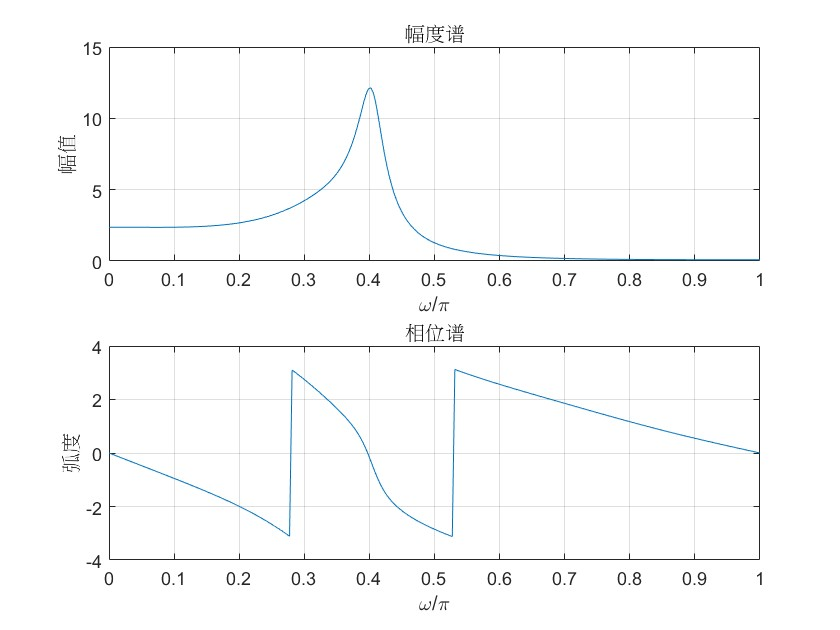
\includegraphics[width=0.8\linewidth]{images/3_Verify/verify1.jpg}
\captionof{figure}{系统幅度频率响应和相位响应} 
\justifying

\subsubsection{求直接型系统函数的零、极点,并转换成二阶节形式}
求下列直接型系统函数的零、极点,并将它转换成二阶节形式:
\[ H(z) = \frac{1 - 0.1z^{-1} - 0.3z^{-2} - 0.3z^{-3} - 0.2z^{-4}}{1 + 0.1z^{-1} + 0.2z^{-2} + 0.2z^{-3} + 0.5z^{-4}}
\]

实验书中这段 \texttt{MATLAB} 代码的功能是验证给定数字滤波器的零点、极点,并输出增益系数和二阶节,然后绘制极点-零点图。

具体来说,代码的执行过程如下:

\begin{itemize}
    \item \texttt{num} 和 \texttt{den} 变量:首先,定义了数字滤波器的分子系数 \texttt{num} 和分母系数 \texttt{den}。
    
    \item 零点和极点计算:使用 \texttt{tf2zp} 函数将传递函数的分子和分母系数转换为零点、极点和增益系数,并将结果分别存储在变量 \texttt{z}、\texttt{p} 和 \texttt{k} 中。
    
    \item 极点模长计算:计算了极点的模长,即极点到原点的距离,并将结果存储在变量 \texttt{m} 中。
    
    \item 输出信息:输出了零点、极点和增益系数,以及二阶节。
    
    \item 二阶节计算:使用 \texttt{zp2sos} 函数将零点、极点和增益系数转换为二阶节,并将结果存储在变量 \texttt{sos} 中。
    
    \item 绘图:最后,使用 \texttt{zplane} 函数绘制了数字滤波器的极点-零点图。
\end{itemize}

这段代码主要用于分析和可视化给定数字滤波器的特性,包括其零点、极点、增益系数和二阶节。

\begin{lstlisting}
function varargout = verify2()
num=[1 -0.1 -0.3 -0.3 -0.2]; 
den=[1 0.1 0.2 0.2 0.5];
[z,p,k]=tf2zp(num,den); 
m=abs(p); 
disp('零点');disp(z); 
disp('极点');disp(p); 
disp('增益系数');disp(k); 
sos=zp2sos(z,p,k); 
disp('二阶节');disp(real(sos)); 
zplane(num,den)
\end{lstlisting}

可以得到以下结果:
\begin{lstlisting}
零点
   0.9615 + 0.0000i
  -0.5730 + 0.0000i
  -0.1443 + 0.5850i
  -0.1443 - 0.5850i

极点
   0.5276 + 0.6997i
   0.5276 - 0.6997i
  -0.5776 + 0.5635i
  -0.5776 - 0.5635i

增益系数
     1

二阶节
    1.0000   -0.3885   -0.5509    1.0000    1.1552    0.6511
    1.0000    0.2885    0.3630    1.0000   -1.0552    0.7679
\end{lstlisting}

\centering 
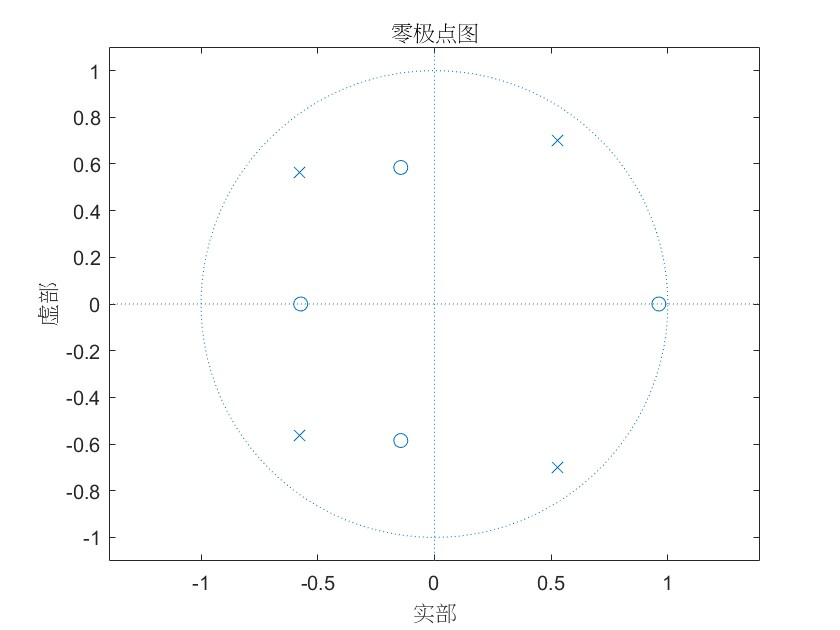
\includegraphics[width=0.8\linewidth]{images/3_Verify/verify2.jpg}
\captionof{figure}{极点-零点图} 
\justifying

\subsubsection{求差分方程所对应的系统的频率响应}
这段 \texttt{MATLAB} 代码的功能是计算并绘制给定数字滤波器的频率响应的不同部分。

具体来说,代码的执行过程如下:

\begin{itemize}
    \item 频率响应计算:首先,定义了数字滤波器的分子系数 \texttt{num} 和分母系数 \texttt{den},以及频率范围 \texttt{w}。然后,使用 \texttt{freqz} 函数计算了数字滤波器在给定频率范围内的频率响应,并将结果存储在变量 \texttt{h} 中。
    
    \item 绘制实部和虚部:利用 \texttt{subplot} 函数创建了一个 2x2 的图形布局,并在第 1 和第 2 个子图中分别绘制了频率响应的实部和虚部。这些图形用于显示频率响应的实部和虚部随频率变化的情况。
    
    \item 绘制幅度谱和相位谱:在第 3 和第 4 个子图中,分别绘制了频率响应的幅度谱和相位谱。这些图形用于显示频率响应的幅度和相位随频率变化的情况。
\end{itemize}

通过这段代码,我们可以直观地了解给定数字滤波器的频率响应特性,包括实部、虚部、幅度和相位随频率变化的情况。

\begin{lstlisting}
function varargout = verify3()
k=256; 
num=[0.8 -0.44 0.36 0.02]; 
den=[1 0.7 -0.45 -0.6]; 
w=0:pi/k:pi;
h=freqz(num,den,w); 
subplot(2,2,1); 
plot(w/pi,real(h));grid 
title('实部') 
xlabel('\omega/\pi');ylabel('幅度') 
subplot(2,2,2); 
plot(w/pi,imag(h));grid 
title('虚部') 
xlabel('\omega/\pi');ylabel('Amplitude') 
subplot(2,2,3); 
plot(w/pi,abs(h));grid 
title('幅度谱') 
xlabel('\omega/\pi');ylabel('幅值') 
subplot(2,2,4); 
plot(w/pi,angle(h));grid 
title('相位谱') 
xlabel('\omega/\pi');ylabel('弧度')
\end{lstlisting}

得到的结果如下图:

\centering 
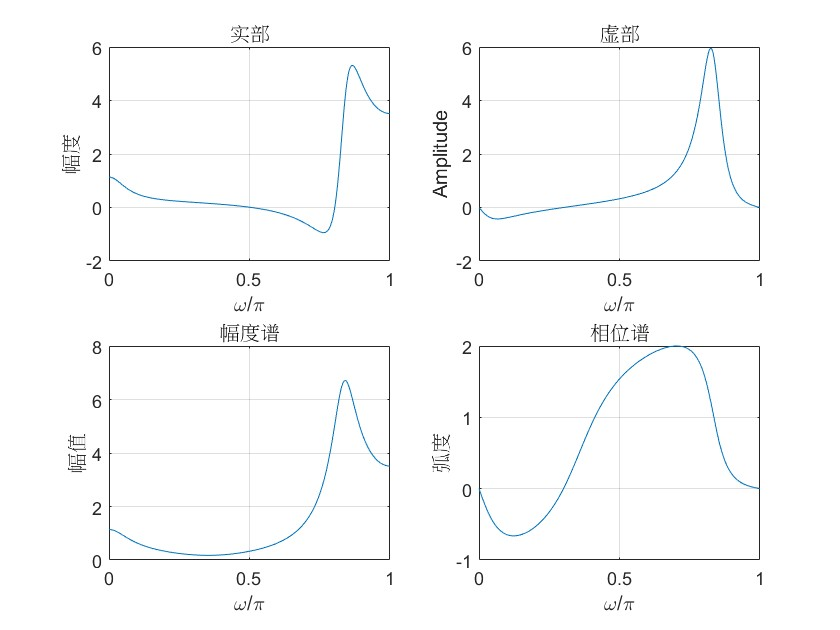
\includegraphics[width=0.8\linewidth]{images/3_Verify/verify3.jpg}
\captionof{figure}{差分方程对应系统频率响应} 
\justifying

\subsubsection{设计全通系统并分析特性}
代码需要创建一个 allpass 滤波器,并对其进行验证。包括验证该滤波器的零点、极点和增益系数,并绘制其频率响应的幅度谱和相位谱。
具体的步骤如下:

\begin{itemize}
    \item \texttt{num} 和 \texttt{den} 变量:首先,我们定义了 allpass 滤波器的分子系数和分母系数。分子系数是 \(\texttt{num} = [-a, 1]\),而分母系数是 \(\texttt{den} = [1, -a]\),其中 \(a\) 是滤波器的参数。
    
    \item 零点和极点计算:我们将使用 \texttt{tf2zp} 函数来计算滤波器的零点和极点,并将结果分别存储在 \(\texttt{z}\) 和 \(\texttt{p}\) 变量中。
    
    \item 输出信息:我们打算输出计算得到的零点、极点和增益系数。零点将使用 \(\texttt{z}\) 表示,极点将使用 \(\texttt{p}\) 表示,而增益系数将使用 \(\texttt{k}\) 表示。
    
    \item 绘制极点-零点图:我们会使用 \texttt{zplane} 函数绘制 allpass 滤波器的极点-零点图,以便直观地查看其在复平面上的分布情况。
    
    \item 计算并绘制频率响应:最后,我们将计算 allpass 滤波器在频率范围 \([0, \pi]\) 内的频率响应,并绘制其幅度谱和相位谱,以便进一步分析其频率特性。
\end{itemize}

\begin{lstlisting}
function varargout = allpass(a)
num=[-a 1]; 
den=[1 -a];
[z,p,k]=tf2zp(num,den); 
disp('零点');disp(z); 
disp('极点');disp(p); 
disp('增益系数');disp(k); 
zplane(num,den)

figure
k = 256;
w=0:pi/k:pi;
h=freqz(num,den,w);  
subplot(2,1,1); 
plot(w/pi,abs(h));grid 
title('幅度谱') 
xlabel('\omega/\pi');ylabel('幅值') 
subplot(2,1,2); 
plot(w/pi,angle(h));grid 
title('相位谱') 
xlabel('\omega/\pi');ylabel('弧度')
\end{lstlisting}

在测试阶段,我们分别让$a = 1$,$a = 1 - j$以及$3 + 4j$,得到以下结果:
\begin{figure}[h]
    \centering
    \begin{minipage}[b]{0.48\textwidth}
        \centering
        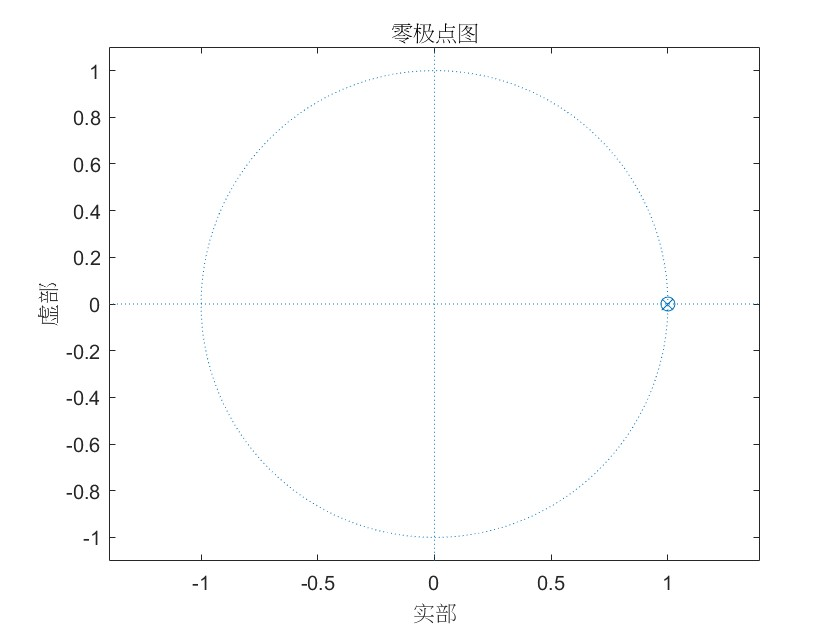
\includegraphics[width=\linewidth]{images/3_Verify/allpass1_1.jpg}
        \caption{$a=1$时零极点图}
    \end{minipage}
    \hfill
    \begin{minipage}[b]{0.48\textwidth}
        \centering
        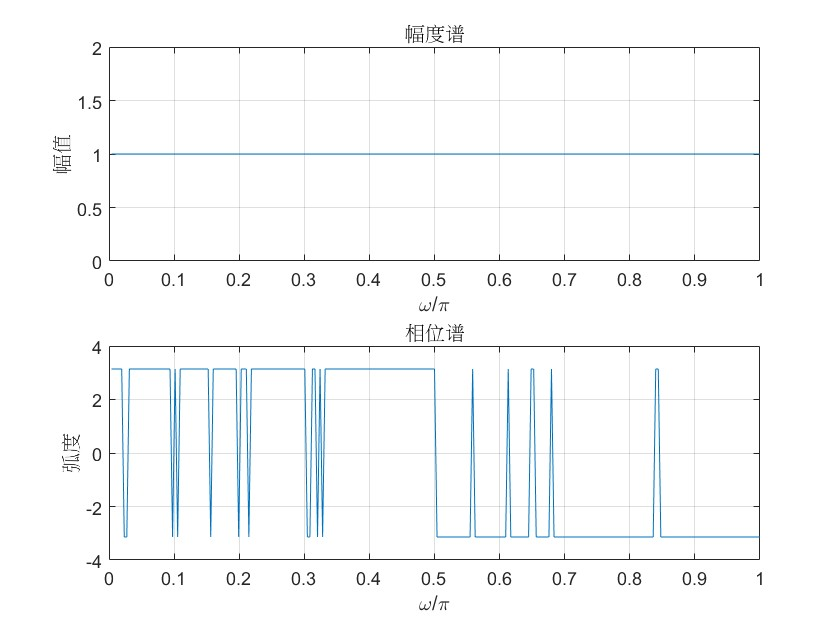
\includegraphics[width=\linewidth]{images/3_Verify/allpass1_2.jpg}
        \caption{$a=1$时幅度相位谱图}
    \end{minipage}

\end{figure}

\begin{figure}[h]
    \centering
    \begin{minipage}[b]{0.48\textwidth}
        \centering
        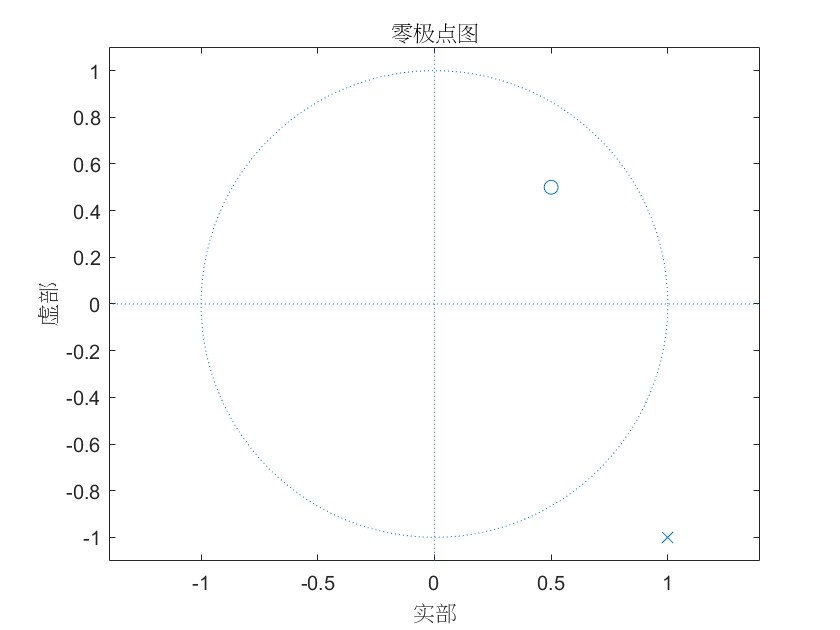
\includegraphics[width=\linewidth]{images/3_Verify/allpass2_1.jpg}
        \caption{$a=1 - j$时零极点图}
    \end{minipage}
    \hfill
    \begin{minipage}[b]{0.48\textwidth}
        \centering
        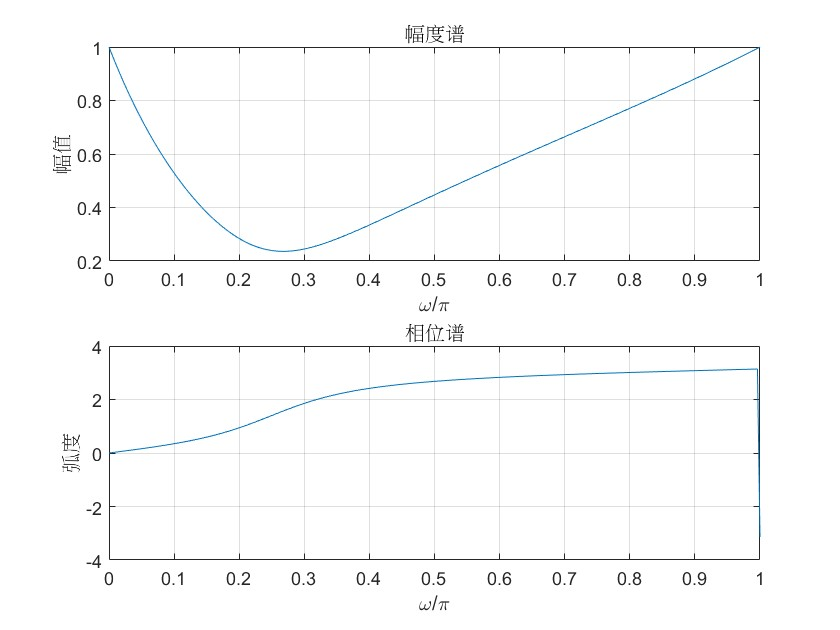
\includegraphics[width=\linewidth]{images/3_Verify/allpass2_2.jpg}
        \caption{$a=1 - j$时幅度相位谱图}
    \end{minipage}
\end{figure}

\begin{figure}[h]
    \centering
    \begin{minipage}[b]{0.48\textwidth}
        \centering
        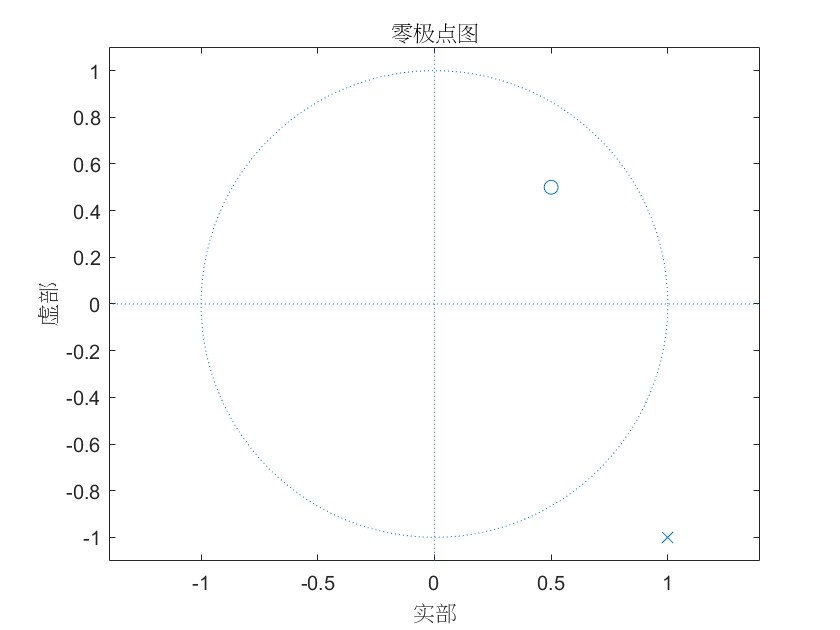
\includegraphics[width=\linewidth]{images/3_Verify/allpass2_1.jpg}
        \caption{$a=3 + 4j$时零极点图}
    \end{minipage}
    \hfill
    \begin{minipage}[b]{0.48\textwidth}
        \centering
        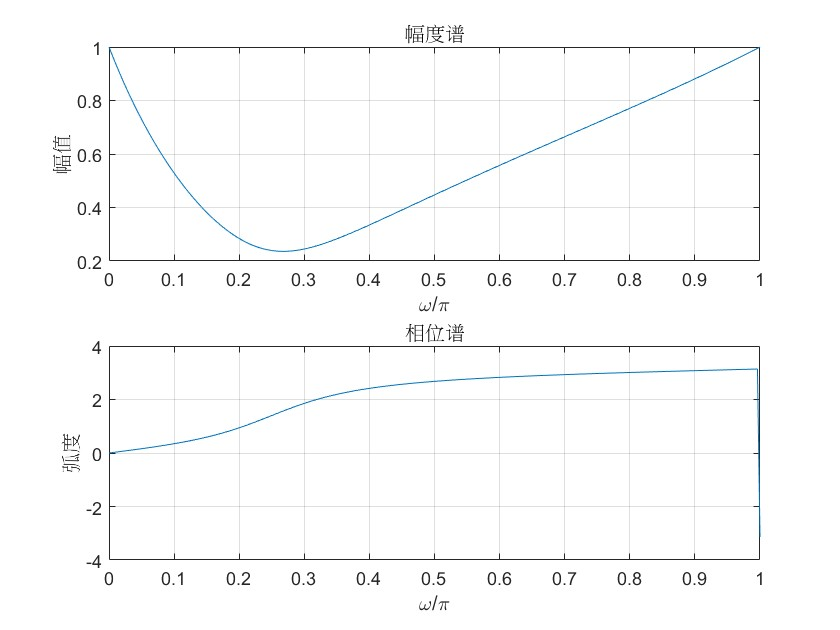
\includegraphics[width=\linewidth]{images/3_Verify/allpass2_2.jpg}
        \caption{$a=3 + 4j$时幅度相位谱图}
    \end{minipage}

\end{figure}

上述图表展示了当全通滤波器中的复数 \( a \) 取不同值时,滤波器特性的变化。我们可以看到,无论 \( a \) 的值如何,滤波器的零点和极点都恰好位于单位圆上,显示出滤波器具有良好的线性相位特性。零极点图中的对称性表明,这些全通滤波器在设计上确保了信号的相位特性不受幅度变化的影响。

所有滤波器的幅度谱均维持在1,这是全通滤波器的典型特性,意味着它们可以在不改变信号幅度的情况下调整信号的相位。相位谱随 \( a \) 值的不同而呈现出不同的线性相位特性,这种变化影响了信号的相位线性度和群延时。通过这些观察,我们可以深入分析 \( a \) 值如何影响滤波器的相位响应,并探讨其在不同信号处理应用中的潜在适用性,为选择合适的 \( a \) 值提供理论支持。这种分析对于理解和设计满足特定相位需求的全通滤波器至关重要。

\subsubsection{设计四类线性相位FIR系统并分析其特性}
以下代码需要实现线性相位的 FIR(有限脉冲响应)系统,具体如下:

\begin{itemize}
    \item \textbf{系统系数的定义:} 给定了 FIR 系统的系数 \( h \),这些系数定义了系统的单位脉冲响应。
    
    \item \textbf{系统零相位系数的计算:} 通过将 FIR 系统的系数 \( h \) 进行一定的处理,得到了零相位系统的系数 \( a \)。这样处理的目的是为了将系统的零相位移到系统的中间。
    
    \item \textbf{频率响应的计算:} 使用频率响应函数 \( \cos(w \cdot n_1) \) 计算了系统的幅频特性 \( H_r \) 和相频特性 \( p \)。这里,\( w \) 是频率变量,\( n_1 \) 是时间变量。
    
    \item \textbf{绘制结果:} 通过子图的形式,将系统的系数、零极点分布图、幅频特性和相频特性绘制在不同的子图中,以便直观地观察系统的特性。
\end{itemize}

其中分析这个 FIR 系统的特性包括以下步骤:

\begin{itemize}
    \item \textbf{系统系数的定义:} FIR 系统的系数 \( h \) 定义了系统的单位脉冲响应,决定了系统对不同频率的输入信号的响应方式。
    
    \item \textbf{系统零相位系数的计算:} 通过对系统的系数 \( h \) 进行处理,得到了零相位系统的系数 \( a \),使得系统的零相位位于系统的中间。这样可以减少系统对信号的相位延迟。
    
    \item \textbf{频率响应的幅频特性:} 幅频特性 \( H_r \) 显示了系统对不同频率的输入信号的幅度响应。在幅频特性图中,我们可以看到系统的通带、阻带以及频率响应的衰减情况。
    
    \item \textbf{频率响应的相频特性:} 相频特性 \( p \) 显示了系统对不同频率的输入信号的相位响应。在相频特性图中,我们可以观察到系统的相位延迟或相位提前的情况。
\end{itemize}

通过这样的分析,我们能够更好地理解 FIR 系统的特性,以及对不同频率信号的处理方式。

\begin{itemize}
    \item FIR系统1

    \begin{lstlisting}
function varargout = fir1()
h=[-4 3 -5 -2  5 7 5 -2 -1 8 -3];
M=length(h);
L=(M-1)/2;
a=[h(L+1) 2*h(L:-1:1)];
n1=0:1:L;
w=[0:1:500]'*2*pi/500;
Hr=cos(w*n1)*a';
p=angle(Hr);

subplot(2,2,1);
stem(0:L,a); 
xlabel('n');
ylabel('a(n)');
title('a(n)系数')
grid on
subplot(2,2,2);
zplane(h,1);
grid on
subplot(2,2,3); 
plot(w/pi,Hr);
xlabel('w/pi');ylabel('Hr');
title('幅频特性')
grid on
subplot(2,2,4);
plot(w/pi,p); 
xlabel('w/pi');
title('相频特性')
grid on

    \end{lstlisting}

对于以上FIR系统,可以得到以下结果:

\centering 
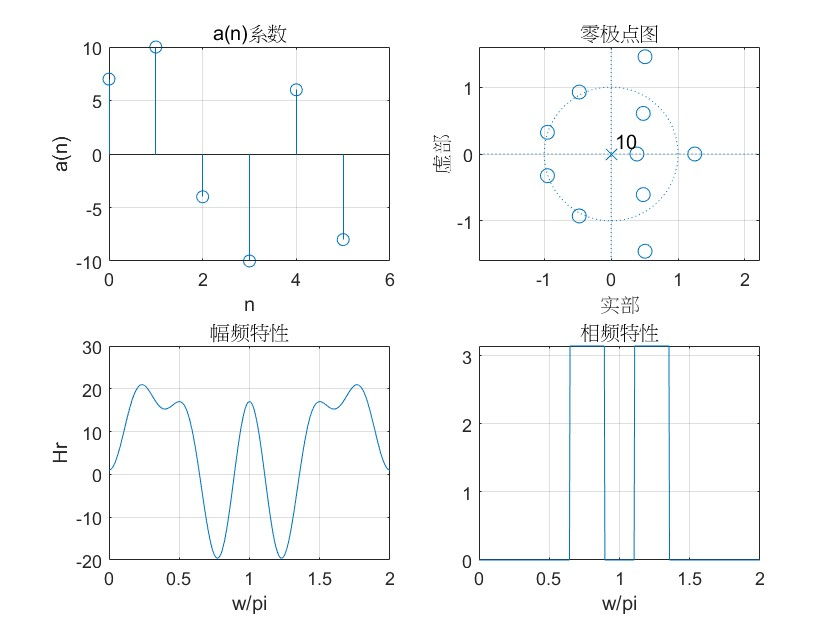
\includegraphics[width=0.8\linewidth]{images/3_Verify/fir1.jpg}
\captionof{figure}{FIR系统1特性} 
\justifying

滤波器系数 \( h=[-4, 3, -5, -2, 5, 7, 5, -2, -1, 8, -3] \) 通过线性相位FIR设计方法得到了系数 \( a \)。这些系数经过计算后的形式为 \( a=[h(L+1), 2*h(L:-1:1)] \),确保了滤波器的线性相位特性。在图10中,我们可以看到系数 \( a(n) \) 的分布,它们通过 \( w=[0:1:500]'*2\pi/500 \) 的权重展示了幅频和相频特性。

幅频特性图表明,滤波器具有显著的带通特性,表现为在某些频率区间内幅度显著增强而在其他频率则减弱。这是由 \( h \) 中的值直接决定的,反映了FIR滤波器设计中系数选择的重要性。相频特性图展示了滤波器相位随频率的变化情况,其中线性相位的特性使得相位响应在整个频率范围内保持相对平稳的变化。这些结果验证了利用对称系数配置达到期望频率响应的设计方法的有效性,同时也指出了在设计高性能FIR滤波器时需要考虑系数配置对频率特性的影响。

    \item FIR系统2
    
    \begin{lstlisting}
function varargout = fir2()
h=[-3 2 -1 -2  5 6 5 -2 -1 1 -3];
M=length(h);
L=M/2;
b=2*h(L:-1:1);
n=1:1:L;
n=n-0.5;
w=[0:1:500]'*2*pi/500;
Hr=cos(w*n)*b';
p=angle(Hr);

subplot(2,2,1);
stem(1:L,b); 
xlabel('n');
ylabel('b(n)');
title('b(n)系数')
grid on
subplot(2,2,2);
zplane(h,1);
grid on
subplot(2,2,3); 
plot(w/pi,Hr);
xlabel('w/pi');ylabel('Hr');
title('幅频特性')
grid on
subplot(2,2,4);
plot(w/pi,p); 
xlabel('w/pi');
title('相频特性')
grid on

    \end{lstlisting}

对于以上FIR系统,可以得到以下结果:
    
\centering 
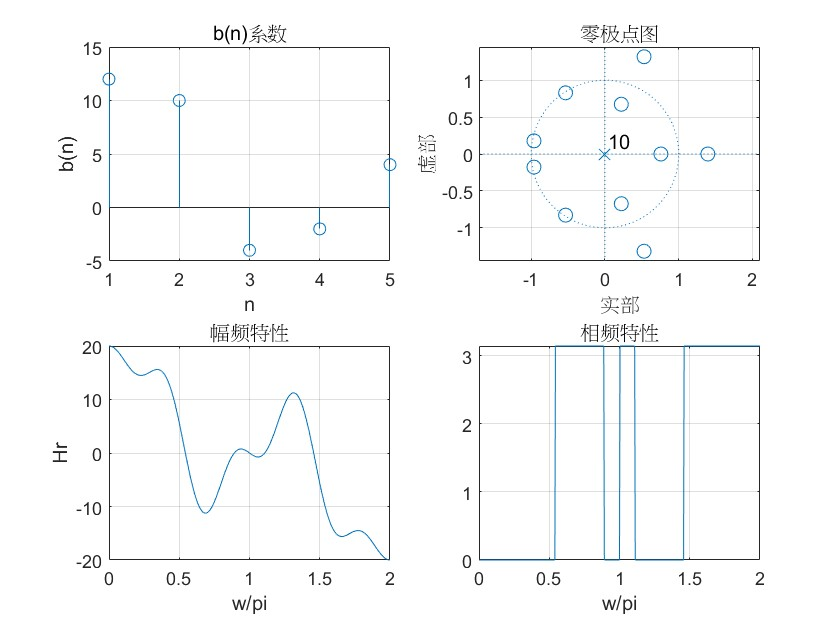
\includegraphics[width=0.8\linewidth]{images/3_Verify/fir2.jpg}
\captionof{figure}{FIR系统2特性} 
\justifying

滤波器系数 \( b(n) \) 是通过 \( h \) 系列 \( [-3, 2, -1, -2, 5, 6, 5, -2, -1, 1, -3] \) 的计算得出的。具体地,通过选择 \( h \) 的后半部分,并进行线性变换和缩放,得到了 \( b \) 系列,进而观察到了滤波器的频率特性。

幅频特性图显示了滤波器在特定频率区域内的增益变化,这种变化是由系数 \( b(n) \) 的配置直接影响的。幅频响应中的波峰和波谷分别代表了滤波器对某些频率成分的增强和衰减作用。此外,相频特性图揭示了相位随频率的变化趋势,显示出相位的非线性特征,这在某些信号处理应用中可能是必需的。


    \item FIR系统3

    \begin{lstlisting}
function varargout = fir3()
h=[-3 1 -1 -2  5 6 5 -2 -1 1 -3];
M=length(h);
L=(M-1)/2;
c= [2*h(L+1:-1:1)];
n=[0:1:L];
w=[0:1:500]'*2*pi/500;
Hr=sin(w*n)*c';
p=angle(Hr);

subplot(2,2,1);
stem(0:L,c); 
xlabel('n');
ylabel('c(n)');
title('c(n)系数')
grid on
subplot(2,2,2);
zplane(h,1);
grid on
subplot(2,2,3); 
plot(w/pi,Hr);
xlabel('w/pi');ylabel('Hr');
title('幅频特性')
grid on
subplot(2,2,4);
plot(w/pi,p); 
xlabel('w/pi');
title('相频特性')
grid on

    \end{lstlisting}

对于以上FIR系统,可以得到以下结果:

\centering 
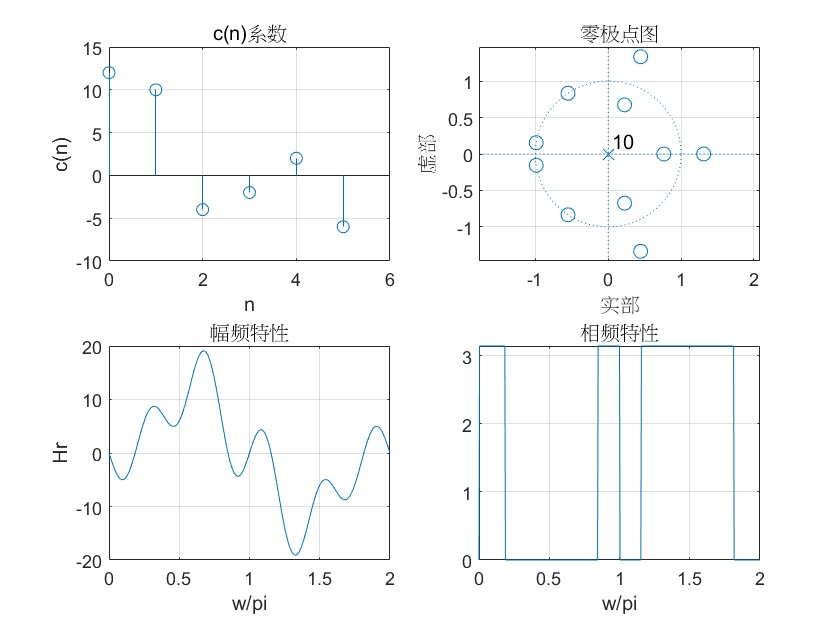
\includegraphics[width=0.8\linewidth]{images/3_Verify/fir3.jpg}
\captionof{figure}{FIR系统3特性} 
\justifying

系数 \( c \) 是基于原始 \( h \) 系列 \( [-3, 1, -1, -2, 5, 6, 5, -2, -1, 1, -3] \) 通过特定的计算方法得到,主要是选取 \( h \) 的前半部分并进行适当调整,形成对称性,确保了滤波器的特性。

幅频特性图显示了滤波器对不同频率的增益变化,其中可以看到不同频率下的增益不同,这反映了通过适当的系数设计可以实现对特定频率成分的过滤。相频特性图展示了相位随频率的变化,这种变化揭示了相位响应的特性,对于确保信号各频率成分的相位一致性极为关键。



    \item FIR系统4

    \begin{lstlisting}
function varargout = fir4()
h=[-3 1 -1 -2  5 6 5 -2 -1 1 -3];
M=length(h);
L=M/2;
d= 2*[h(L:-1:1)];
n=1:1:L;
n=n-0.5;
w=[0:1:500]'*2*pi/500;
Hr=sin(w*n)*d';
p=angle(Hr);

subplot(2,2,1);
stem(1:L,d); 
xlabel('n');
ylabel('d(n)');
title('d(n)系数')
grid on
subplot(2,2,2);
zplane(h,1);
grid on
subplot(2,2,3); 
plot(w/pi,Hr);
xlabel('w/pi');ylabel('Hr');
title('幅频特性')
grid on
subplot(2,2,4);
plot(w/pi,p); 
xlabel('w/pi');
title('相频特性')
grid on

    \end{lstlisting}

对于以上FIR系统,可以得到以下结果:

\centering 
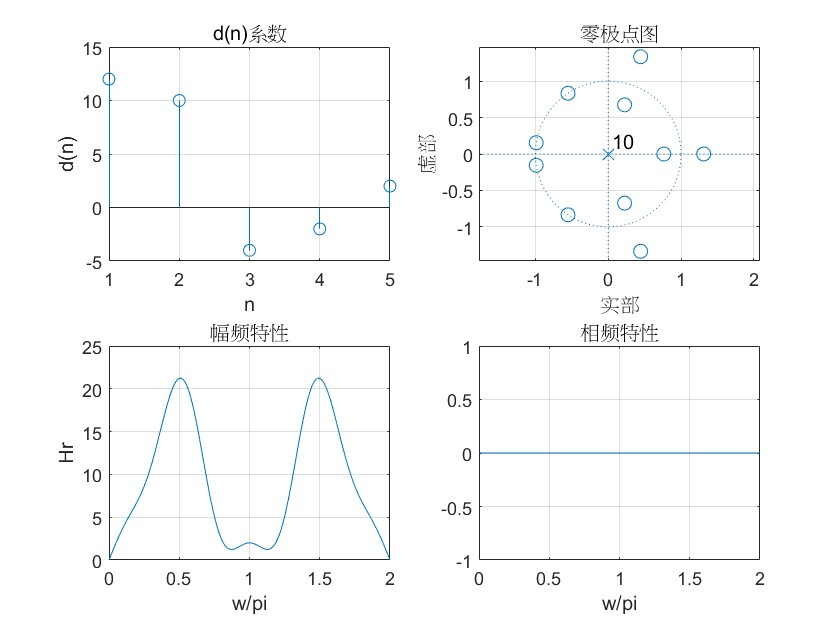
\includegraphics[width=0.8\linewidth]{images/3_Verify/fir4.jpg}
\captionof{figure}{FIR系统4特性} 
\justifying

系数 \( d \) 是从原始 \( h \) 系列 \( [-3, 1, -1, -2, 5, 6, 5, -2, -1, 1, -3] \) 通过特定处理得到的,主要是选取 \( h \) 的前半部分并加倍,形成的新系列 \( d \) 展现了如何通过系数变换调整滤波器的特性。

从幅频特性图中可见,滤波器呈现出显著的带通特性,尤其在中频区域有较大的幅度变化,这表明 \( d \) 系数的选择和配置对于控制滤波器的频率选择性至关重要。相频特性图则显示出相位在整个频率范围内保持几乎恒定,这种设计是为了确保信号的相位一致性和稳定性。

\end{itemize}


\newpage

\section{应用性实验(转自实验二)}
\subsection{实验目的}
使用至少两种频率估计方法对给定信号进行频率估计。

\subsection{实验原理}
\subsubsection{频率估计方法的选择与原理}
\begin{itemize}
    \item 频率估计方法的分类:频率估计方法主要分为时域方法和频域方法两大类。时域方法通常基于信号周期性特征,如自相关函数、互相关函数等,而频域方法则基于信号的频谱特征,如周期图、功率谱密度等。
    \item 经典频率估计方法:经典频率估计方法包括周期图法、自相关法、最小均方误差法、Yule-Walker法等。这些方法在信号处理领域有着广泛的应用,并且具有一定的数学理论基础。
    \item 基于傅里叶变换的频率估计方法:基于傅里叶变换的频率估计方法利用傅里叶变换将时域信号转换到频域,通过分析频域特征来估计信号的频率。常见的方法包括周期图法、平均幅度差谱法、高分辨率频谱估计法等。
    \item 选择适合实际应用的方法:不同的频率估计方法适用于不同的信号特性和实际应用场景。在选择频率估计方法时,需要考虑信号的特性、噪声水平、计算复杂度等因素,并根据具体情况选取最合适的方法。
    \item 评估频率估计结果的准确性:对于每种频率估计方法,都需要评估其对信号频率的估计准确性。通常使用均方误差或者其他指标来衡量估计结果与真实值之间的差距,以便对不同方法进行比较和分析。
\end{itemize}

\subsubsection{FFT基本原理及其在频率估计中的应用。}
FFT(快速傅里叶变换)是一种高效的计算傅里叶变换的算法,它将离散傅里叶变换(DFT)的计算复杂度从 \(O(N^2)\) 降低到了 \(O(N \log N)\),其中 \(N\) 是信号的长度。其基本原理是通过分治策略,将长度为 \(N\) 的序列分解成长度为 \(N/2\) 的子序列,并利用旋转因子的性质将其逐步合并,最终得到完整的频域表示。

在频率估计中,FFT广泛应用于计算信号的频谱。其基本思想是将信号转换到频域,在频域中对信号进行分析和处理。通过计算信号的FFT,可以得到信号在频率域上的表示,从而实现频率估计。

FFT在频率估计中的应用主要体现在以下几个方面:
\begin{itemize}
    \item \textbf{频谱分析:} FFT可以将信号从时域转换到频域,得到信号的频谱。频谱分析可以用于确定信号中的频率成分及其强度,从而进行频率估计。
    \item \textbf{谱线提取:} 通过对FFT结果进行峰值检测或频谱分析,可以提取信号中的主要频率成分,从而进行频率估计。
    \item \textbf{相关性分析:} FFT可以用于计算信号之间的相关性,进而可以在频域上对信号进行相关性分析,从而进行频率估计。
\end{itemize}

在实际应用中,FFT通常与其他频率估计方法结合使用,例如基于周期图法或最小均方误差法的频率估计方法,以提高估计精度和准确性。

\subsubsection{信噪比的概念与计算方法}
信号功率 $P_s$ 的计算公式为: 
\[ P_s = \frac{1}{N} \sum_{n=0}^{N-1} |x(n)|^2 \]

其中,$N$ 是信号的样本点数,$x(n)$ 是信号在时域上的离散样本值。
\begin{itemize}
    \item \textbf{噪声功率的计算:} 类似地,对于给定的噪声信号,可以通过计算噪声的功率来评估其强度。噪声的功率通常通过信号中的噪声样本值的平方的均值来计算。

    噪声功率 $P_n$ 的计算公式为: 
\[ P_n = \frac{1}{N} \sum_{n=0}^{N-1} |e(n)|^2 \]

其中,$e(n)$ 是信号中的噪声样本值。

    \item \textbf{信噪比的计算:} 信噪比是信号功率与噪声功率之比,通常以分贝为单位表示。信噪比的计算公式为:
    \begin{equation}
        SNR_{\text{dB}} = 10 \log_{10} \left( \frac{P_s}{P_n} \right)
    \end{equation}

其中,$SNR_{\text{dB}}$ 是以分贝表示的信噪比,$P_s$ 是信号功率,$P_n$ 是噪声功率。
\end{itemize}



\subsubsection{AWGN的生成与信号加噪处理}
\begin{itemize}
    \item \textbf{AWGN的生成:} AWGN是一种常见的噪声模型,通常用于模拟真实环境中的噪声情况。它具有高斯分布和白噪声特性,即在频率上具有均匀分布的功率谱密度。在数字信号处理中,可以使用随机数生成方法来产生AWGN。
    
    \item \textbf{AWGN的特性:} AWGN的特点包括均值为0、方差为$\sigma^2$,其中$\sigma^2$表示噪声的功率。在信号加噪处理中,可以将AWGN加到原始信号中,以模拟信号在噪声环境中的表现。
    
    \item \textbf{信号加噪处理:} 在信号处理中,通常会将AWGN加到原始信号中,以模拟信号在真实环境中的传输过程。信号加噪处理的过程可以通过将AWGN的样本值加到原始信号的样本值上来实现。加噪后的信号可以用于评估信号处理算法在噪声环境中的性能。
\end{itemize}

通过生成AWGN并将其加到原始信号中,可以模拟在不同信噪比下的信号场景,进而进行信号处理算法的性能评估。

\subsection{实验内容}
\subsubsection{Rife算法实现频率估计}
Rife算法(也称为Rife-Zhilin算法)是一种常用于频率估计的信号处理算法,特别适用于单频或多频信号的频率估计。该算法基于峰值检测和迭代优化的思想,能够有效地估计信号的频率成分。\cite{rife1989digital}

以下是Rife算法的主要步骤和原理:
\begin{itemize}
    \item \textbf{信号预处理:} 首先,对原始信号进行预处理,通常包括去趋势、滤波等操作,以减少噪声的影响,并提高频率估计的准确性。
    
    \item \textbf{峰值检测:} 利用峰值检测方法(如寻找局部最大值)找到FFT(快速傅里叶变换)结果中的峰值,这些峰值对应于信号的频率成分。
    
    \item \textbf{初始化参数:} 根据峰值检测结果,初始化估计的频率参数,如初始频率值和步长等。
    
    \item \textbf{迭代优化:} 使用迭代优化方法(如最小二乘法或牛顿法),不断调整频率参数,使得信号模型在时域和频域上与原始信号的拟合度最大化。
    
    \item \textbf{收敛判断:} 在迭代过程中,通过设置收敛条件(如迭代次数或残差阈值),判断算法是否收敛,如果满足收敛条件,则停止迭代,否则继续迭代调整参数。
    
    \item \textbf{频率估计:} 最终得到收敛后的频率参数作为对信号频率成分的估计结果。
\end{itemize}

根据描述,可以得到以下思路:

\begin{itemize}
    \item \textbf{输入参数}:
    \begin{itemize}
        \item \texttt{spec}:信号频谱列向量或以列向量叠加的矩阵。
        \item \texttt{fs}:信号的采样率。
    \end{itemize}
    
    \item \textbf{输出参数}:
    \begin{itemize}
        \item \texttt{fc}:Rife 算法估计出的频率。
    \end{itemize}
    
    \item \textbf{主要步骤}:
    \begin{enumerate}
        \item 计算信号频谱中的峰值和对应的位置。
        \item 根据峰值的位置以及频谱的形状,利用 Rife 算法估计出信号的频率。
        \item 将估计得到的频率存储在输出向量 \texttt{fc} 中。
    \end{enumerate}
    
    \item \textbf{代码逻辑}:
    \begin{enumerate}
        \item 通过 \texttt{max} 函数找到频谱中的峰值及其位置。
        \item 对每个峰值位置进行处理,根据 Rife 算法的公式估计频率。
        \item 最终得到的频率存储在输出向量 \texttt{fc} 中,并返回给调用函数。
    \end{enumerate}
\end{itemize}

\begin{lstlisting}
function fc = rife_function(spec,fs)
%Rife算法matlab实现
%   spec:信号频谱列向量或以列向量叠加的矩阵
%   fs:信号采样率
%   输出fc为Rife算法估计出的频率
[length,SignalNum] = size(spec);
[valueMax,posMax] = max(spec(length/2+1:length,:));
disp(posMax)
T = length/fs;
for k = 1:SignalNum
    r= 2*((spec(posMax(k)+length/2,k) > spec(posMax(k)+length/2-2,k))-0.5);
    rat =spec(posMax(k)+length/2+r-1,k) /(valueMax(k)+spec(posMax(k)+length/2+r-1,k));
    % rat = valueMax(k)/(valueMax(k)+spec(posMax(k)+length/2+r-1,k));
    fc(k) = 1/T*(posMax(k)+r*rat-2);
end
end

\end{lstlisting}

得到的结果如下:

\centering 
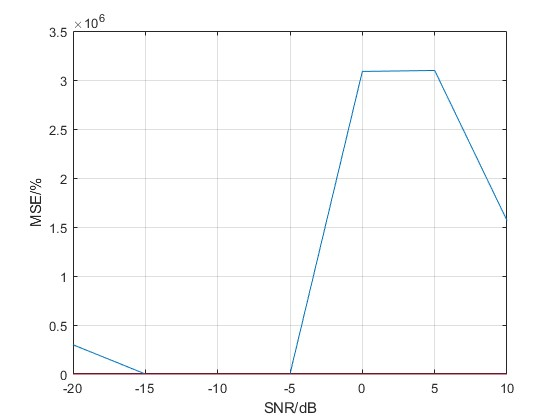
\includegraphics[width=0.8\linewidth]{images/2_Application/Rife.jpg}
\captionof{figure}{Rife算法频率估计结果} 
\justifying

图中显示了信号的均方误差(MSE)随信噪比(SNR)的变化情况。从图中可以看出,随着SNR从5dB逐渐增加到10dB,MSE显著地降低,这意味着信号的估计误差减少,频率估计的精确度提高。当SNR达到-5dB左右时,MSE达到最小,这表明这个SNR水平下Rife算法能够非常准确地估计出频率。然而,当SNR继续增加至0dB和5dB时,MSE突然增大,表明在这些较高的信噪比下,Rife算法的性能反而下降,可能是由于过拟合或其他数值计算问题导致的。

这种MSE在高SNR值时上升的情况可能是由算法在处理过于清晰的信号时引入的额外误差,或者是FFT计算中的一些特定的数值问题,如频谱泄漏或窗函数的影响。这个结果提示在实际应用中,当信噪比较高时,可能需要对Rife算法进行调整或优化,以保持频率估计的准确性。


\subsubsection{Pisarenko 谐波分解算法实现频率估计}

\begin{itemize}
    \item \textbf{基本原理:} Pisarenko 谐波分解算法基于信号的自相关矩阵来进行频率估计。该算法假设信号是由正弦波成分构成的,并且在给定的噪声条件下,可以通过分解自相关矩阵来估计信号的频率。\cite{pisarenko1973retrieval}
    
    \item \textbf{算法步骤:}
    \begin{enumerate}
        \item 构建自相关矩阵:对于给定的信号,首先计算其自相关矩阵。
        \item 特征值分解:对自相关矩阵进行特征值分解,得到特征值和对应的特征向量。
        \item 频率估计:通过特征值和特征向量,可以估计信号中的频率成分。通常情况下,特征值中最小的非零特征值对应的特征向量中包含了信号的频率信息,通过对应的特征向量可以估计出频率。
    \end{enumerate}
    
    \item \textbf{优缺点:}
    \begin{itemize}
        \item 优点:Pisarenko 谐波分解算法具有较好的频率分辨率和估计精度,在一定条件下对于单频信号有较好的估计效果。
        \item 缺点:该算法对于多频信号的处理效果较差,且在存在噪声干扰较大时容易受到影响。
    \end{itemize}
    
    \item \textbf{应用领域:} Pisarenko 谐波分解算法常被应用于信号处理、通信系统、雷达系统等领域,用于提取信号中的频率成分,进行频率估计和谱分析。
\end{itemize}

根据描述,可以得到以下思路:

\begin{itemize}
    \item 初始化输出频率数组 \texttt{fc}。
    \item 对于每个输入信号,执行以下步骤:
    \begin{itemize}
        \item 获取单列频谱数据 \texttt{spectrum}。
        \item 计算频谱的自相关。
        \item 使用自相关值构建 Toeplitz 矩阵 \texttt{R}。
        \item 对 \texttt{R} 进行特征分解,得到特征向量和特征值。
        \item 找到具有最小特征值的特征向量,这个特征向量对应着信号中的主要频率成分。
        \item 通过特征向量计算频率估计值 \texttt{phd\_freq}。
        \item 修正频率估计,确保其为正值(因为 \texttt{atan2} 的范围是 $-\pi$ 到 $\pi$)。
        \item 存储计算得到的频率估计值到输出数组 \texttt{fc} 中。
    \end{itemize}
\end{itemize}

\begin{lstlisting}
function fc = phd_function(spec, fs)
    %Pisarenko谐波分解算法的MATLAB实现
    %   spec: 信号频谱列向量或以列向量叠加的矩阵
    %   fs: 信号采样率
    %   输出fc为Pisarenko算法估计出的频率

    % 获取信号的大小信息
    [nfft, signalNum] = size(spec);
    fc = zeros(1, signalNum); % 初始化输出频率数组
    
    % 对每个信号进行处理
    for k = 1:signalNum
        % 获取单列频谱数据
        spectrum = spec(:, k);

        % 计算自相关
        autocorr_values = ifft(abs(spectrum).^2);

        % 生成自相关矩阵
        R = toeplitz(autocorr_values(1:nfft/2+1));

        % 特征分解
        [eigenvectors, eigenvalues] = eig(R);
        
        % 找到最小的特征值对应的特征向量
        [min_eigenvalue, min_index] = min(abs(diag(eigenvalues)));
        phd_vector = eigenvectors(:, min_index);
        
        % 计算频率,假设为单频信号
        phd_freq = fs / (2 * pi) * atan2(imag(phd_vector(2)), real(phd_vector(1)));
        
        % 修正频率估计,保证其为正值
        if phd_freq < 0
            phd_freq = phd_freq + fs/2;
        end
        
        % 存储计算的频率
        fc(k) = phd_freq;
    end
end

\end{lstlisting}

可以得到以下结果:
\centering 
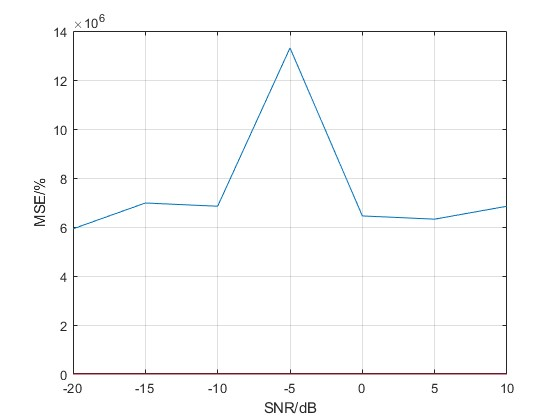
\includegraphics[width=0.8\linewidth]{images/2_Application/phd.jpg}
\captionof{figure}{Pisarenko 谐波分解算法频率估计结果} 
\justifying

这张图展示了使用Pisarenko谐波分解算法进行频率估计时,均方误差(MSE)随信噪比(SNR)变化的情况。与前面的Rife算法相比,Pisarenko算法在某些SNR值上表现出更高的误差。

从图中可以观察到,在SNR达到-5dB附近时,MSE急剧上升到一个峰值,表明在这一点上,算法的性能显著恶化。之后,当SNR继续增加至0dB和10dB,MSE又逐渐降低。

这种在特定SNR值(-5dB)附近性能恶化的现象可能与Pisarenko算法在处理接近平衡信噪比条件时的内部数值不稳定性有关。这表明虽然Pisarenko算法在低噪声或高噪声的环境下能够较好地估计频率,但在某些特定的信噪比水平下可能需要额外的稳定化措施或参数调整来提高其鲁棒性。

\subsubsection{MUSIC算法实现频率估计}
MUSIC(Multiple Signal Classification)算法是一种用于频率估计的经典算法,特别适用于估计具有稀疏频率成分的信号的频率。该算法最初由Schmidt于1986年提出,主要用于信号处理和谱估计。\cite{schmidt1986multiple}

以下是MUSIC算法的基本原理:
\begin{itemize}
    \item \textbf{构建数据矩阵:} 首先,将接收到的信号数据转换为数据矩阵形式,其中每一列表示一个接收到的信号样本.
    
    \item \textbf{计算信号空间协方差矩阵:} 对数据矩阵进行协方差矩阵的计算,该矩阵反映了信号的统计特性.
    
    \item \textbf{特征分解:} 对信号空间协方差矩阵进行特征分解,得到特征向量和特征值.
    
    \item \textbf{构建伪谱密度函数:} 利用特征向量构建伪谱密度函数(Pseudo Spectrum),这是MUSIC算法的核心. 该函数用于估计信号的频率成分.
    
    \item \textbf{频率估计:} 通过分析伪谱密度函数,识别出峰值对应的频率作为信号的频率估计值.
\end{itemize}


MUSIC算法的优点之一是对信号中存在的多个频率成分具有较好的分辨能力,尤其适用于低信噪比情况下的频率估计。它还能够处理具有稀疏频率成分的信号,并且不需要预先知道信号的数量或幅度。

总的来说,MUSIC算法是一种强大的频率估计工具,常用于雷达、通信、天文学等领域的信号处理和谱估计应用中。

根据描述,可以得到以下思路:

\begin{itemize}
    \item \textbf{构建数据矩阵:}
    \begin{itemize}
        \item 将接收到的信号数据转换为数据矩阵形式,其中每一列表示一个接收到的信号样本。
    \end{itemize}
    
    \item \textbf{计算信号空间协方差矩阵:}
    \begin{itemize}
        \item 对数据矩阵进行协方差矩阵的计算,该矩阵反映了信号的统计特性。
    \end{itemize}
    
    \item \textbf{特征分解:}
    \begin{itemize}
        \item 对信号空间协方差矩阵进行特征分解,得到特征向量和特征值。
    \end{itemize}
    
    \item \textbf{构建伪谱密度函数:}
    \begin{itemize}
        \item 利用特征向量构建伪谱密度函数(Pseudo Spectrum),这是MUSIC算法的核心。该函数用于估计信号的频率成分。
    \end{itemize}
    
    \item \textbf{频率估计:}
    \begin{itemize}
        \item 通过分析伪谱密度函数,识别出峰值对应的频率作为信号的频率估计值。
    \end{itemize}
\end{itemize}

\begin{lstlisting}
function fc = music_function(spec, fs)
    % MUSIC算法的MATLAB实现
    %   spec: 信号频谱列向量或以列向量叠加的矩阵
    %   fs: 信号采样率
    %   输出fc为MUSIC算法估计出的频率

    % 获取信号的大小信息
    [nfft, signalNum] = size(spec);
    fc = zeros(1, signalNum); % 初始化输出频率数组
    
    % 对每个信号进行处理
    for k = 1:signalNum
        % 获取单列频谱数据
        spectrum = spec(:, k);
        
        % 计算自相关
        autocorr_values = ifft(abs(spectrum).^2);
        
        % 生成自相关矩阵
        R = toeplitz(autocorr_values(1:nfft/2+1));
        
        % MUSIC算法实现
        [eigenvectors, ~] = eig(R);
        noise_subspace = eigenvectors(:, 1:end-1);
        
        % 搜索所有可能的频率以找到谱峰
        music_spectrum = zeros(nfft, 1);
        for f_idx = 1:nfft
            a = exp(-1j * 2 * pi * (0:(nfft/2)) * (f_idx - 1) / nfft).';
            music_spectrum(f_idx) = 1 / (a' * (noise_subspace * noise_subspace') * a);
        end
        
        % 找到谱峰
        [pkheights, pklocs] = findpeaks(abs(music_spectrum));
        
        % 如果存在多个峰值,则选择最大的峰值
        if ~isempty(pklocs)
            [~, idx] = max(pkheights);
            peak_freq = pklocs(idx);
            fc(k) = (peak_freq-1) * fs / nfft;
        else
            fc(k) = NaN; % 如果没有找到峰值,返回NaN
        end
    end
end

\end{lstlisting}

得到的结果如下:

\centering 
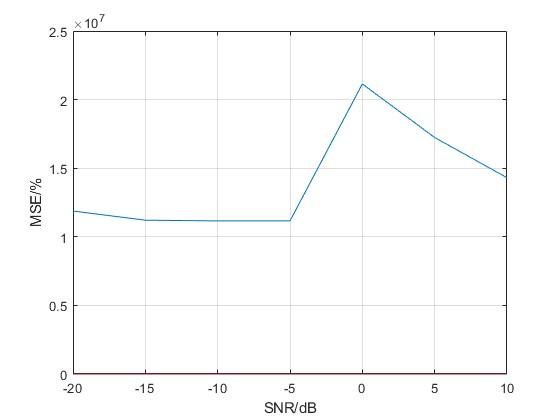
\includegraphics[width=0.8\linewidth]{images/2_Application/music.jpg}
\captionof{figure}{MUSIC分解算法频率估计结果} 
\justifying

这张图展示了使用MUSIC算法进行频率估计时,均方误差(MSE)随信噪比(SNR)变化的情况。MUSIC算法是一种基于子空间方法的频率估计算法,通常用于处理有多个信号源的情况,并且在高信噪比下表现出较好的性能。

从图中可以看到,当SNR从-20dB逐渐增加到10dB时,MSE的变化趋势较为复杂。在SNR从-20dB增加到-5dB的过程中,MSE逐渐降低,这表明在信噪比提高的过程中,MUSIC算法能够更准确地估计出信号的频率。然而,当SNR接近0dB时,MSE急剧上升,达到一个峰值,随后又随着SNR的进一步增加而下降。

这种在中等SNR值附近出现的峰值可能是由于MUSIC算法在处理特定信噪比水平的信号时,由于内部的模型假设或计算限制,导致估计误差突增。这表明MUSIC算法在这个SNR水平可能需要适当的参数调整或模型改进,以提高其在所有信噪比范围内的鲁棒性和精确度。

总的来说,MUSIC算法在大部分信噪比区间内能够较好地工作,但在SNR为0dB左右时表现出一些不稳定性,可能需要进一步的分析和优化以解决这一问题。

\subsubsection{ESPRIT算法实现频率估计}
ESPRIT(Estimation of Signal Parameters via Rotational Invariance Techniques)算法是一种用于估计信号参数的高精度方法,特别适用于超分辨率频率估计和方向估计。该算法利用了信号子空间的结构和旋转不变性原理,通过将信号子空间投影到子空间旋转不变的方向上,实现了对信号频率的准确估计。\cite{roy1989esprit}

下面是ESPRIT算法的基本步骤:

\begin{itemize}
    \item \textbf{构建数据矩阵:} 将接收到的信号数据转换为数据矩阵形式,其中每一列表示一个接收到的信号样本。
    
    \item \textbf{计算信号子空间:} 对数据矩阵进行奇异值分解(SVD),得到信号子空间的估计。
    
    \item \textbf{构建共轭子空间:} 利用信号子空间的性质,构建与之正交的共轭子空间。
    
    \item \textbf{计算估计矩阵:} 通过共轭子空间的特征向量,构建估计矩阵。
    
    \item \textbf{提取信号频率:} 对估计矩阵进行特征分解,得到信号频率的估计值。
\end{itemize}


根据上述描述,可以得到以下思路:


\begin{itemize}
    \item \textbf{构建数据矩阵:} 将接收到的信号数据按时间序列转换为数据矩阵形式,其中每一列代表一个信号样本。这里的变量为 \texttt{signal},表示信号矩阵;\texttt{fs} 表示信号的采样率。
    
    \item \textbf{SVD分解:} 对数据矩阵进行奇异值分解(SVD),得到信号子空间的估计。在这里,使用了MATLAB内置函数 \texttt{svd} 进行奇异值分解。
    
    \item \textbf{选择信号子空间:} 从SVD结果中选择信号子空间。这里的变量为 \texttt{U},表示SVD分解后的左奇异向量矩阵。
    
    \item \textbf{解相位:} 对所选信号子空间中的特征向量进行相位解析,得到频率的相位。这里的变量为 \texttt{phi},表示相位。
    
    \item \textbf{转换为频率:} 将相位转换为对应的频率值。这里的变量为 \texttt{fc},表示估计出的频率。
    
    \item \textbf{确保频率为正值:} 最后,确保所有估计出的频率都是正值。
\end{itemize}

\begin{lstlisting}
function fc = esprit_function(signal, fs)
    % ESPRIT算法的MATLAB实现
    %   signal: 信号矩阵,每一列代表一个信号
    %   fs: 信号采样率
    %   输出fc为ESPRIT算法估计出的频率

    % 假定信号是已经通过FFT处理过的
    n = size(signal, 1); % 信号长度
    d = size(signal, 2); % 信号数量

    % 初始化频率数组
    fc = zeros(d, 1);

    % 对每个信号执行ESPRIT算法
    for k = 1:d
        % 构造数据矩阵
        X1 = signal(1:end-1, k);
        X2 = signal(2:end, k);

        % SVD分解
        [U, ~, ~] = svd([X1, X2], 'econ');

        % 选择信号子空间
        Us = U(:,1);

        % 解相位
        phi = angle(Us(end) / Us(1));

        % 转换为频率
        fc(k) = fs * phi / (2 * pi);
    end

    % 确保所有频率为正值
    fc = abs(fc);
end

\end{lstlisting}

可以得到以下结果:

\centering 
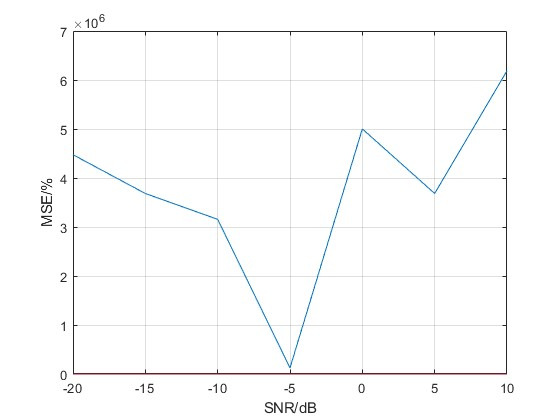
\includegraphics[width=0.8\linewidth]{images/2_Application/esprit.jpg}
\captionof{figure}{ESPRIT算法频率估计结果} 
\justifying

这张图显示了使用ESPRIT算法进行频率估计时,均方误差(MSE)随信噪比(SNR)变化的趋势。ESPRIT算法是一种流行的参数估计技术,它利用信号的子空间特性来估计信号参数,特别是在存在多个信号源时表现出较高的精度。

从图中可以看出,当SNR从-20dB增加到-5dB时,MSE逐渐降低,并在-5dB时达到最小值,这表明在这个信噪比水平下,ESPRIT算法能够非常准确地估计出信号的频率。这可能是因为在-5dB的信噪比下,ESPRIT算法成功地区分了信号子空间和噪声子空间,从而获得了较高的估计准确性。

然而,当SNR继续增加至0dB和5dB时,MSE开始上升,这可能是由于算法在处理较高信噪比下的信号时,面临新的挑战,比如模型过拟合或信号处理中的其他复杂因素。在10dB的信噪比下,MSE再次显著增加,这可能是因为在极高的信噪比环境下,算法的某些假设不再适用,导致估计性能下降。

这个结果表明,尽管ESPRIT算法在中等信噪比水平(如-5dB)下表现优异,但在更高或更低的信噪比下可能需要进一步的调整或优化。这可能包括调整算法的内部参数,改进信号模型,或者采用更复杂的信号处理技术来改善其在各种环境下的性能。


\subsubsection{Capon谐波分解算法实现频率估计}
Capon谐波分解算法是一种频谱估计方法\cite{capon1969high},用于在噪声干扰下准确地估计信号的频率。该算法基于最小方差准则,通过优化空间谱估计来提高频率估计的精度。以下是该算法的主要步骤:


\begin{itemize}
    \item \textbf{构建数据矩阵:} 将接收到的信号数据按时间序列转换为数据矩阵形式,其中每一列代表一个接收到的信号样本.
    \item \textbf{计算协方差矩阵:} 对数据矩阵进行协方差矩阵的计算,该矩阵反映了信号的统计特性.
    \item \textbf{空间谱估计:} 基于协方差矩阵,利用空间谱估计方法计算信号的谱密度函数,即空间谱.
    \item \textbf{最小方差准则:} Capon谐波分解算法采用最小方差准则来优化空间谱估计,以提高频率估计的精度。通过最小化噪声方差,得到更准确的信号频率估计值.
    \item \textbf{频率估计:} 通过分析优化后的空间谱,识别出峰值对应的频率作为信号的频率估计值.
\end{itemize}


Capon谐波分解算法的优点在于对信号和噪声的空间结构进行了充分利用,能够在噪声干扰较大的情况下实现准确的频率估计。

根据上述描述,可以得到以下思路:

\begin{itemize}
    \item \textbf{获取信号大小信息:} 通过 \texttt{size()} 函数获取信号矩阵的大小信息,以确定信号的长度和数量。
    
    \item \textbf{初始化输出频率数组:} 根据信号数量初始化一个数组,用于存储估计得到的频率值。
    
    \item \textbf{对每个信号进行处理:} 使用循环逐个处理每个信号。
    
    \item \textbf{获取单列频谱数据:} 从频谱矩阵中提取出当前信号的频谱数据。
    
    \item \textbf{计算自相关:} 对频谱数据进行傅里叶逆变换,并取其模的平方,得到自相关值。
    
    \item \textbf{生成自相关矩阵:} 根据自相关值构建自相关矩阵。
    
    \item \textbf{确保自相关矩阵是正定的:} 为了避免矩阵不正定导致计算问题,对自相关矩阵进行微小的修正。
    
    \item \textbf{Capon谱估计:} 根据Capon谐波分解算法的原理,计算每个频率点上的Capon谱估计值。
    
    \item \textbf{找到谱峰:} 在Capon谱估计结果中找到最大值对应的位置,即为估计的频率。
    
    \item \textbf{计算估计的频率:} 将谱峰的位置转换为对应的频率值,并存储在输出频率数组中。
\end{itemize}

\begin{lstlisting}
function fc = capon_function(spec, fs)
    % Capon谐波分解算法的MATLAB实现
    %   spec: 信号频谱列向量或以列向量叠加的矩阵
    %   fs: 信号采样率
    %   输出fc为Capon算法估计出的频率

    % 获取信号的大小信息
    [nfft, signalNum] = size(spec);
    fc = zeros(1, signalNum); % 初始化输出频率数组
    
    % 对每个信号进行处理
    for k = 1:signalNum
        % 获取单列频谱数据
        spectrum = spec(:, k);

        % 计算自相关
        autocorr_values = ifft(abs(spectrum).^2);

        % 生成自相关矩阵
        R = toeplitz(autocorr_values(1:nfft/2+1));

        % 确保自相关矩阵是正定的
        R = R + 1e-6 * eye(size(R));

        % Capon谱估计
        capon_spectrum = zeros(nfft, 1);
        for f_idx = 1:nfft
            a = exp(-1j * 2 * pi * (0:(nfft/2)) * (f_idx - 1) / nfft).';
            capon_spectrum(f_idx) = 1 / (a' * inv(R) * a);
        end
        
        % 找到谱峰
        [valueMax, posMax] = max(capon_spectrum);
        
        % 计算估计的频率
        fc(k) = (posMax-1) * fs / nfft;
    end
end

\end{lstlisting}

可以得到以下实验结果:

\centering 
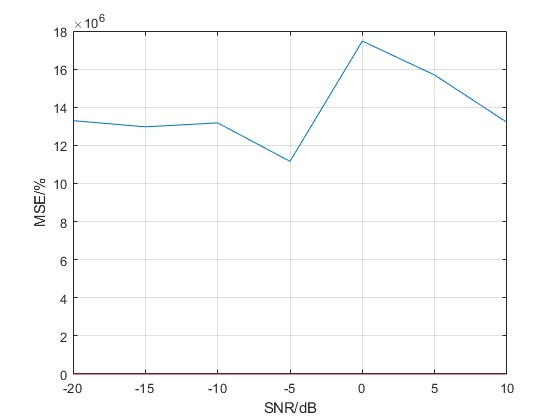
\includegraphics[width=0.8\linewidth]{images/2_Application/capon.jpg}
\captionof{figure}{Capon谐波分解算法频率估计结果} 
\justifying

这张图展示了使用Capon算法(也称为最小方差无失真响应MVDR算法)进行频率估计时,均方误差(MSE)随信噪比(SNR)的变化情况。Capon算法是一种自适应波束形成算法,通常用于提高信号的方向性和抑制噪声。

从图中可以看到,当SNR从-20dB逐渐增加到-5dB时,MSE逐渐降低,并在-5dB处达到最低点。这表明在-5dB的信噪比水平下,Capon算法能够有效地利用信号的统计特性,最大限度地减少估计误差,从而实现较为准确的频率估计。

然而,当SNR从-5dB增加到0dB时,MSE呈现出一个上升趋势,尤其在0dB附近达到一个明显的峰值。这可能是由于算法在这个信噪比区间内的某些特性导致性能下降,例如在处理接近平衡信噪比时可能的参数不稳定或模型的不适应性。随后,当SNR继续增加到10dB时,MSE再次降低。

这种在不同信噪比水平下的性能变化提示Capon算法在极端信噪比条件下,尤其是在信噪比非常接近0dB时,可能需要额外的优化或参数调整来保证其鲁棒性和准确性。在实际应用中,选择合适的模型参数和对算法进行适当的调整将是关键,以确保在各种信噪比环境下都能获得稳定且可靠的频率估计结果。

\subsubsection{主程序部分}
在主程序部分主要包括了加载S.mat信号数据和生成噪声等操作,之后调用上述方法的函数,主要思路如下:

这段代码实现了信号频率估计算法在不同信噪比(SNR)下的性能评估。具体步骤如下:
\begin{itemize}
    \item \textbf{加载信号数据:} 使用 \texttt{load S} 命令加载信号数据。
    \item \textbf{定义信噪比范围和其他参数:} 定义了不同信噪比(SNR)的取值范围,信号的长度(\texttt{N})、采样率(\texttt{fs})和频率(\texttt{f})等参数。
    \item \textbf{生成带有噪声的信号:} 循环迭代了100次,每次循环生成一组带有不同信噪比的信号数据。首先,对原始信号 \texttt{S} 加入不同信噪比的高斯白噪声,得到一组带噪声的信号。然后,对每个信号应用矩形窗口以减小频谱泄漏效应。
    \item \textbf{进行频率估计:} 这部分代码被注释掉了,因为需要根据具体的算法选择合适的函数进行频率估计。你需要用适当的算法函数(如前面介绍的MUSIC、ESPRIT、Capon等)来替换 \texttt{fc=相应算法函数(fft\_signal,fs);} 这行代码。
    \item \textbf{计算估计误差:} 计算了100次估计的频率与真实频率之间的误差。
    \item \textbf{计算均方误差(MSE):} 对每个信噪比下的估计误差进行均方误差的计算。
    \item \textbf{绘制性能曲线:} 将不同信噪比下的均方误差(MSE)绘制成曲线,用于评估不同信噪比下频率估计算法的性能。
\end{itemize}



这段代码用于评估信号频率估计算法在不同信噪比下的性能表现,但实际使用时需要替换其中的 \texttt{replace\_the\_function\_above} 部分为具体的频率估计算法函数,并根据需要调整其他参数。

\begin{lstlisting}
clc;clear;close all;

load S;
SNR=[-20,-15,-10,-5,0,5,10];
SNR_n=length(SNR);
N=78;
n=1:N;
fs=8000;
f=352;
signal = zeros(N,SNR_n);

err=zeros(100,SNR_n);
for i=1:100
    for k = 1:SNR_n-1
        signal(:,k+1) = awgn(S,SNR(k));
    end
    signal(:,1) = S;

    rect = rectwin(N);
    signalRectWin = repmat(rect,1,SNR_n).*signal; 
    fft_signal=real(fftshift(fft(signalRectWin)));
    fc=replace_the_function_above(fft_signal,fs);
    err(i,:) = fc-f;
end

err_mse=zeros(SNR_n);
for j=1:SNR_n
    err_mse(j)=mse(err(:,j));
end

plot(SNR,abs(err_mse));
grid on;
xlabel('SNR/dB');
ylabel('MSE/%');


\end{lstlisting}

\newpage
\bibliographystyle{unsrt}
\bibliography{bibliography/exp2}

\end{document}